\subsection{Langsam zeitlich veränderliche Ströme}

Auf- und Entladen eines Kondensators

\paragraph{a.) Aufladen} \hfill \\

$ I(t) $? : $ U_C(t) $?

\begin{center}
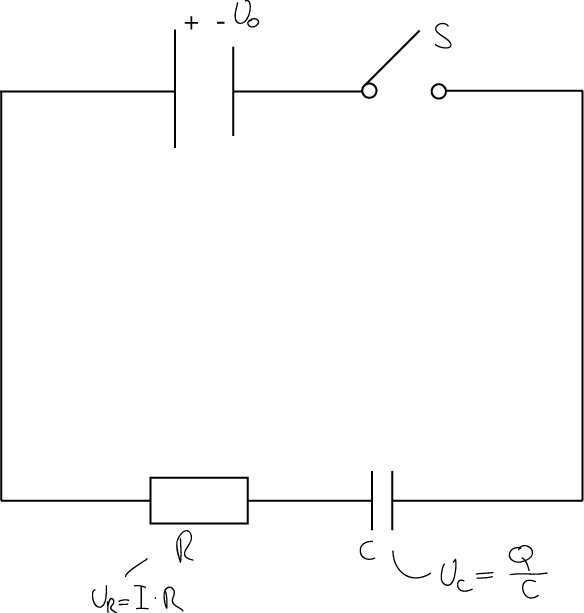
\includegraphics[width=0.4\linewidth]{skizzen/15/15_7/1}
\end{center}


S schließen bei $ t=0 $

	\subparagraph{Maschenregel:}
		\begin{align*}
			U_0& = U_R+U_C = I(t) \cdot R + C^{-1} \cdot Q(t)  \hspace{5mm} | \cdot \frac{d}{dt} \\
			\frac{d}{dt} U_0 &=R \cdot \dot{I}(t) + C^{-1} \frac{dQ(t)}{dt} \\
			\iff 0 &= C^{-1} \cdot I(t) + R \cdot \dot{I}(t) 
		\end{align*}
		DGL für I(t): $ \boxed{\dot{I}(t) + \frac{1}{RC} I(t) = 0} $ \\
		
	\subparagraph{Lösung der DGL durch Separation der Variabeln:}\hfill \\
		\begin{align*}
		\frac{dI(t)}{dt} &= - \frac{1}{RC} I(t)\\
		\frac{dI(t)}{I(t)} &= - \frac{1}{RC} \cdot dt \\
		\Rightarrow \int \frac{dI(t)}{I} &= - \frac{1}{RC} \int dt \\
		\ln I(t) &= - \frac{1}{RC} \cdot t + \underline{const} \\
		&= - \frac{t}{RC} + \underline{\ln I_0} \\
		\end{align*}
		$$\ln\frac{I(t)}{I_0} = -\frac{t}{RC}$$ \\ 
		$$\underline{\underline{\Rightarrow I(t) = I_0 \cdot \exp(-\frac{t}{RC})}}$$
		
	Anfangsbedingungen: $ t=0 $ : $ U_C = 0 $ ; $ U_0 = I_0 \cdot R $ \\
	$$ I(t=0) = I_0 = \frac{U_0}{R}  $$ \\
	außerdem $ I (t\rightarrow\infty) = 0 $ (Kondensator aufgeladen) \\
	$ \tau=RC $: Relaxationszeit: [$ \tau $] $ = \frac{V}{A} \cdot \frac{As}{V} = s $ \\
	("\emph{RC-Konstante}") \\
	\hfill \\
	Spannung am Kondensator:
	\begin{flalign*}
	U_C(t) &= U_0 - U_R = U_0 - R \cdot I (t) = I_0 \cdot R - R \cdot I(t)\\
	&=U_0(1-\exp(-t/RC)) \hspace{5mm} \text{mit } U_0=I_0 \cdot R\\
	\hfill \\
	t=0 &: U_C=0\\
	t=\tau &: U_C(t) = (1-e^{-1}) \cdot U_0 \\
	t\rightarrow\infty &: U_C \rightarrow U_0
	\end{flalign*}
	
	\begin{center}
		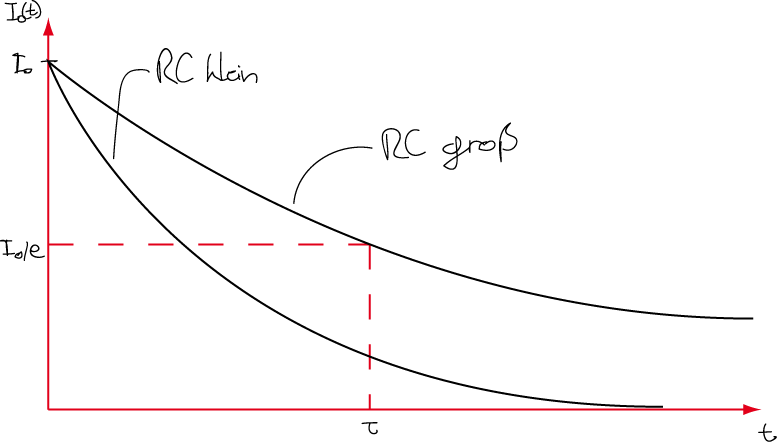
\includegraphics[width=0.6\linewidth]{skizzen/15/15_7/2}
	\end{center}

	
	\begin{center}
		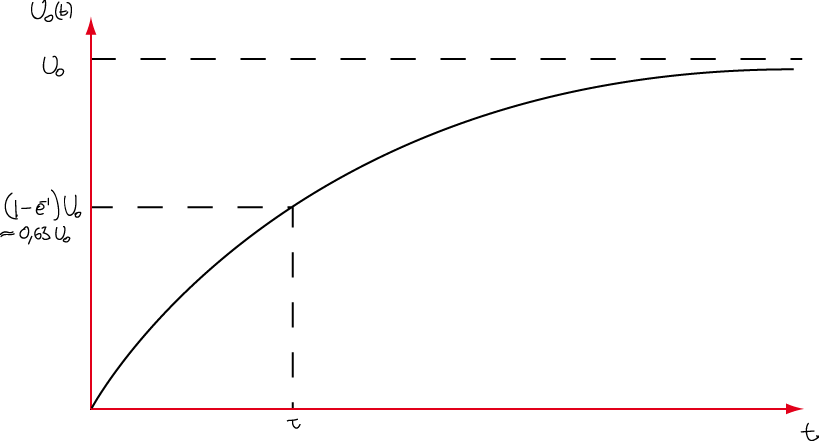
\includegraphics[width=0.6\linewidth]{skizzen/15/15_7/3}
	\end{center}

	
	$ C=\underset{100\si{\micro\farad}}{200\si{\micro\farad}} $ ; $ R=2,6\si{\kilo\ohm} $ ; $ \tau \approx \underset{0,25\si{\second}}{0,5\si{\second}} $ \\
	
\paragraph{b.) Entladen} \hfill \\
	$ I(t) $? : $ U_C(t) $? \\
	\begin{center}
		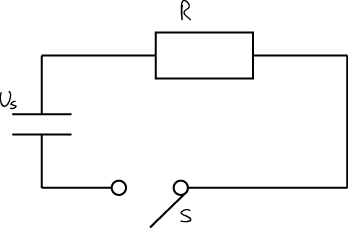
\includegraphics[width=0.4\linewidth]{skizzen/15/15_7/4}
	\end{center}

	2.KG: \\
	$ U_R + U_C = 0 $ (Keine EMK!)\\
	$ \underbracket{I(t)}_{\frac{dQ}{dt}} \cdot R = -\frac{Q(t)}{C} $ \\
	$ \frac{dQ(t)}{Q(t)} = -\frac{1}{RC} dt $ \\
	Lösung: \\
	$\Rightarrow  Q(t) = Q_0 \cdot \exp(-t(RC)^{-1}) $ \\
	$ \Rightarrow I(t) = \frac{dQ(t)}{dt} = -\frac{Q_0}{RC} \cdot \exp(-t(RC)^{-1}) $\\
	$ U_C(t) = -U_R(t) = \frac{Q_0}{C} \cdot \exp(-t(RC)^{-1}) $ \\
	\begin{center}
		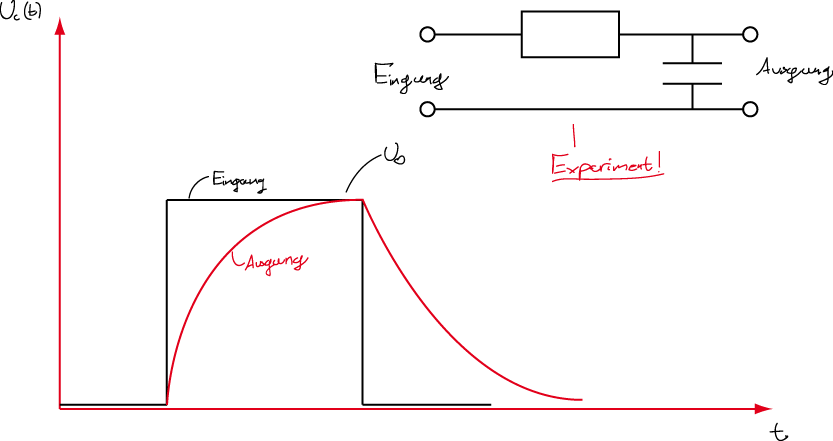
\includegraphics[width=0.6\linewidth]{skizzen/15/15_7/5}
	\end{center}

		